\documentclass{beamer}
\usetheme[subsectionpage=progressbar, background=white]{metropolis}
\usepackage[utf8]{inputenc}
\usepackage{graphicx,color}
\usepackage{amsfonts}
\usepackage{amsmath}
\usepackage{amssymb}
\usepackage{verbatim}
\usepackage{fancyhdr}
\usepackage{epigraph}
\usepackage{caption}
\usepackage{psfrag}
\usepackage{afterpage}
\usepackage[backend=biber, style=nature]{biblatex}
\addbibresource{../bibTex/thesis-library.bib}
\useinnertheme{circles}
\graphicspath{{../figures/}}
%\setbeamercovered{transparent}
\newcommand{\Note}[1]{{\bf \color{red}#1}}    %Anotaciones
\newcommand{\esc}{\!\cdot\!}
\newcommand{\llangle}{\left\langle}
\newcommand{\rrangle}{\right\rangle}
\newcommand{\llg}{\left\lgroup}
\newcommand{\rlg}{\right\rgroup}
\newcommand{\bra}{\llbracket}
\newcommand{\ket}{\rrbracket}
\newcommand{\cc}{\!\parallel\!}
\newcommand{\GK}[2]{\langle#1 \cc #2\rangle}
\newcommand{\GKrest}[2]{\langle#1 \cc #2\rangle^0}

\title{Nanoscale hydrodynamics near solids}
\date{July 2019}
\author{Diego Duque Zumajo}
\institute{Departamento Física Fundamental \\Universidad Nacional de Educación a Distancia}

% logo of my university
\titlegraphic{%
\begin{picture}(0,0)
\put(308,-119){\makebox(0,0)[rt]{
\includegraphics[width=1.5cm]{logo}}}
\end{picture}}

\begin{document}
\maketitle

\begin{frame}{Motivation}
  \begin{itemize}
    \item Great interest in the study of fluids in contact with solids in the nanoscale.
        \item Density layering $\rightarrow$ DFT for equilibrium situations $\rightarrow$ DDFT for the study of the dynamic behaviour of the fluid. 
        \item Slip boundary condition
          \begin{align}
            \delta\frac{\partial v}{\partial z}=v_{\rm slip}, && \delta =\frac{\eta}{\gamma} \nonumber
          \end{align}
        \item Bocquet and Barrat \cite{Bocquet1993}
\begin{align}
  \gamma=\frac{1}{Sk_BT}\int_0^{\tau} dt \llangle \hat{F}^x(t)\hat{F}^x\rrangle
\nonumber
\end{align}
      \item Petravic and Harrowell \cite{Petravic2007} disagree with the expression obtained by Bocquet and Barrat.
      \item The expression for $\gamma$ suffers from the plateau problem. 
    \end{itemize}
\end{frame}

\begin{frame}{Roadmap}
  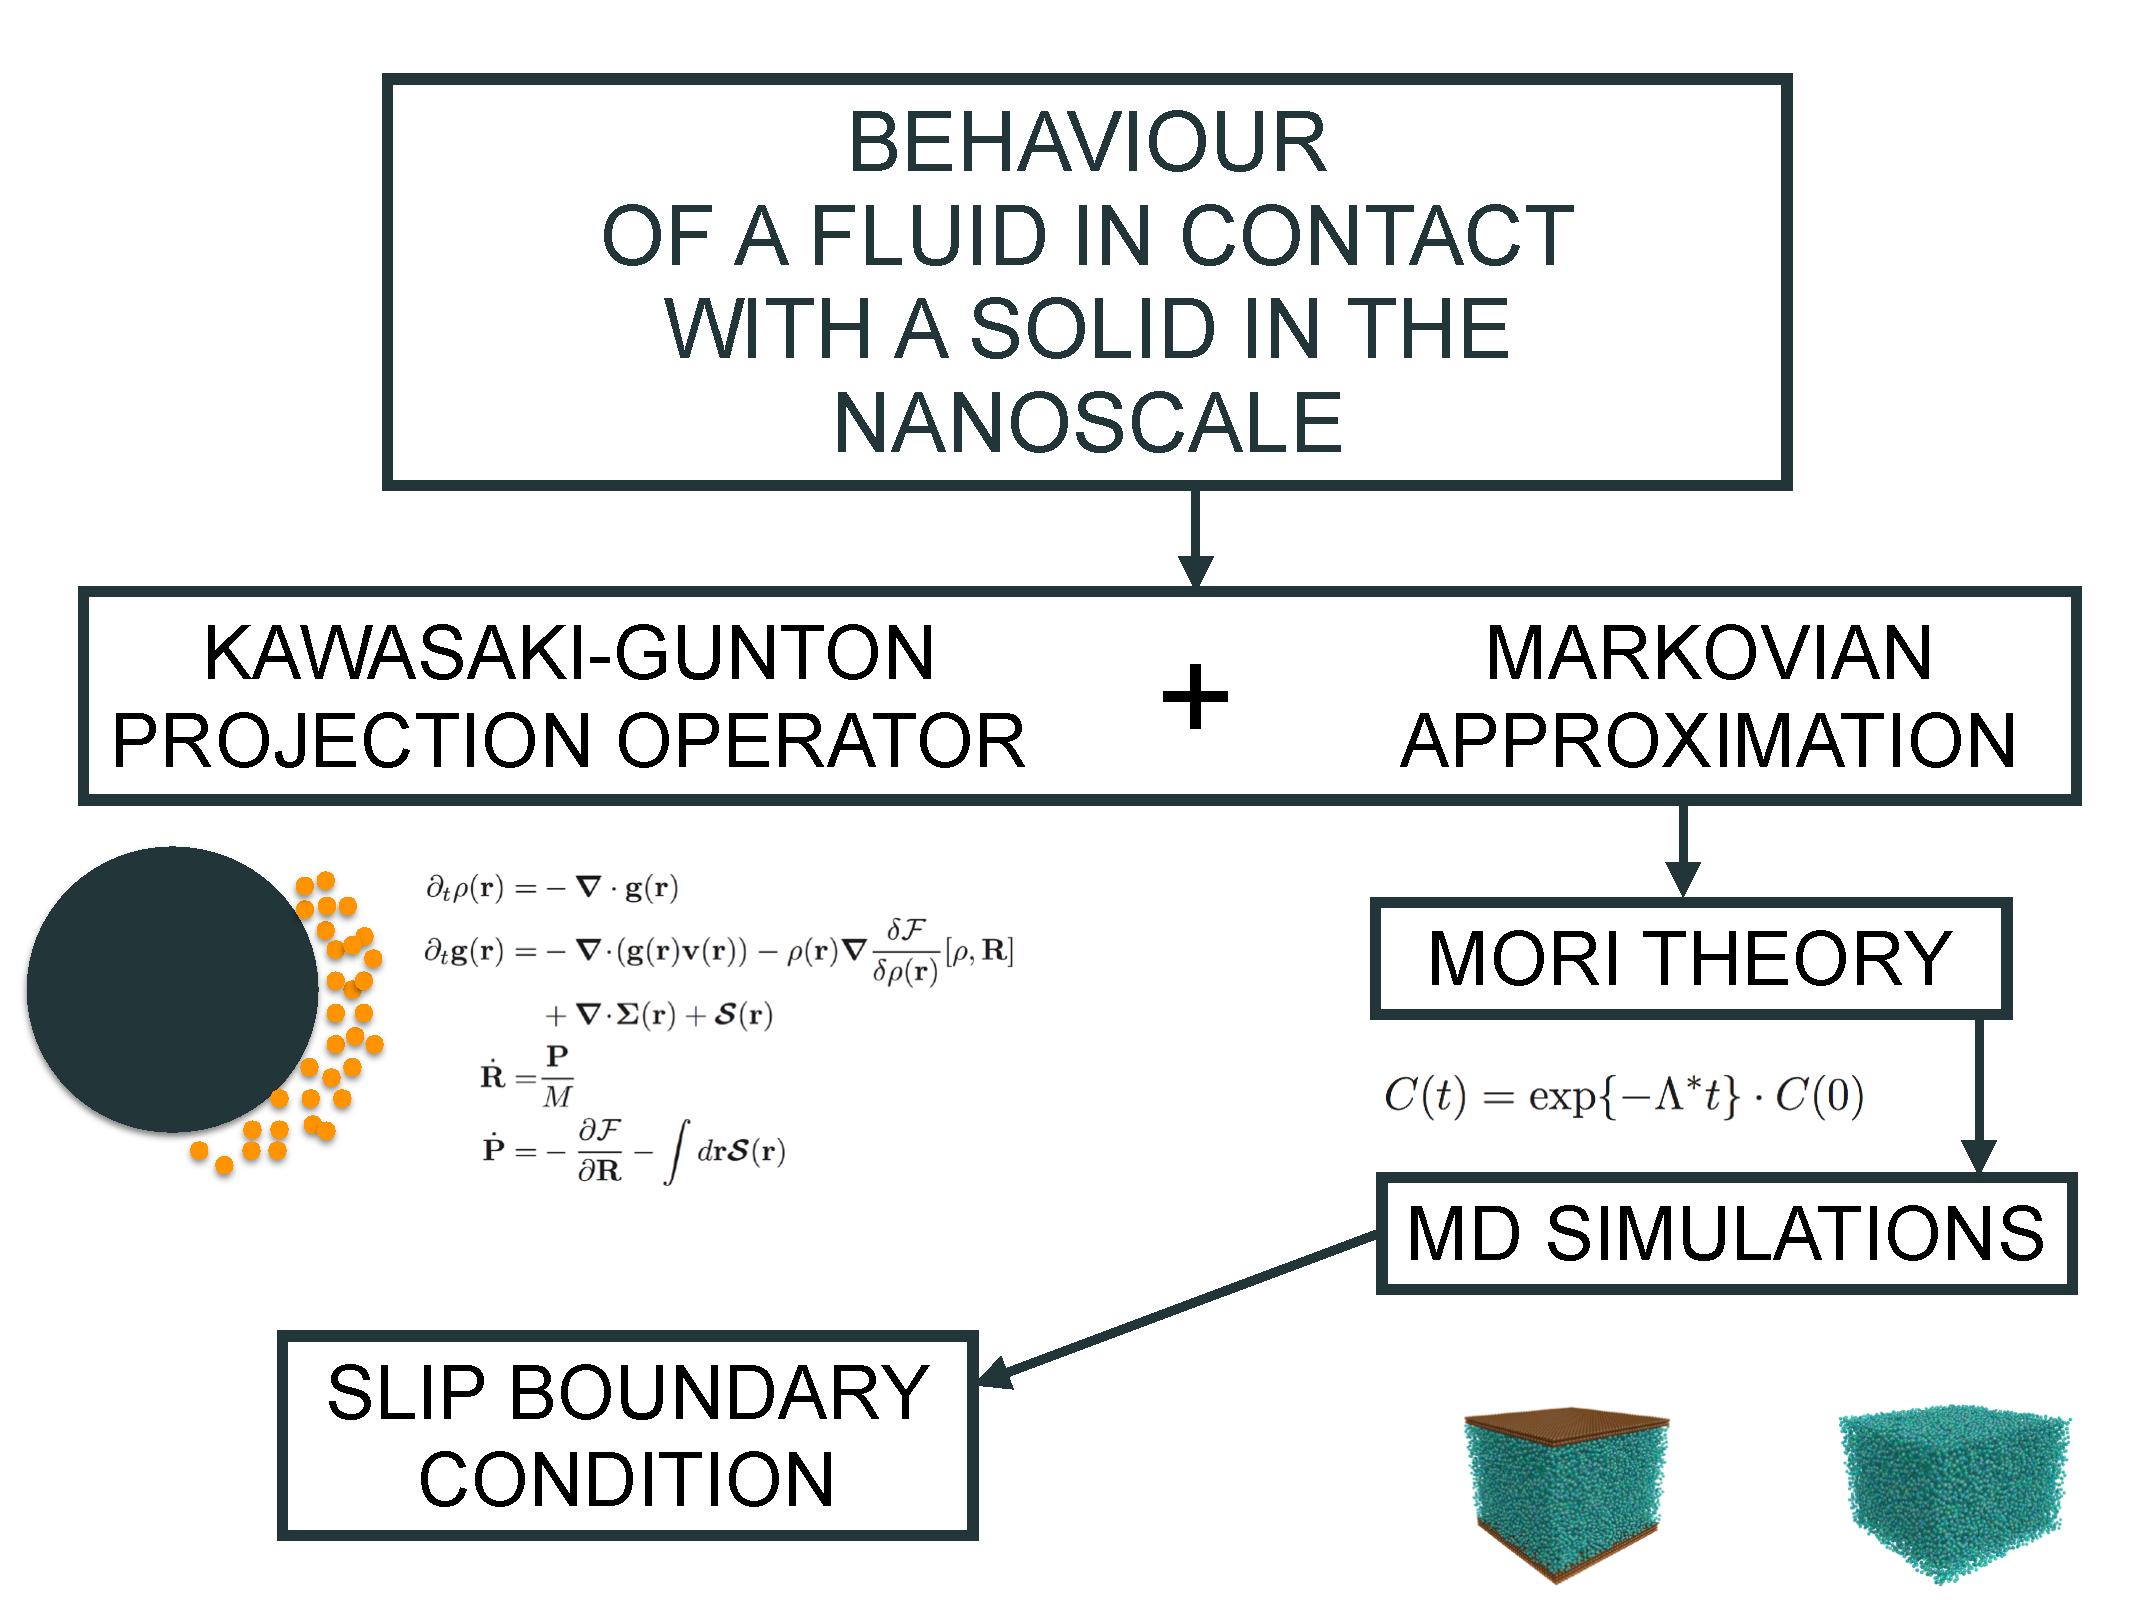
\includegraphics[width=\linewidth]{scheme-thesis}
\end{frame}

\section{Hydrodynamics theory for liquids near solids}
\begin{frame}{The system and the relevant variables}
  \begin{itemize}
    \item We study a fluid with $N$ particles in contact with a solid sphere of $N'$ particles.
    \item $z= ({\bf q}_i, {\bf p}_i)$ and $z'= ({\bf q}_{i'}, {\bf p}_{i'})$
    \item The relevant variables 
      \begin{align}
        \hat{\rho}_{\bf r}(z) &=\sum^{N}_im\delta({\bf r}-{\bf q}_i)
      &&\hat{\bf R}(z)=\frac{1}{N'}\sum_{i'}^{N'}{\bf q}_{i'}
      \nonumber\\
        \hat{\bf g}_{\bf r}(z) &=\sum^{N}_i{\bf p}_i\delta({\bf r}-{\bf q}_i)
      &&\hat{\bf P}(z)=\sum_{i'}^{N'}{\bf p}_{i'}
      \nonumber
      \end{align}
    \item The derivatives of the relevant variables
      \begin{align}
        i{\cal L} \hat{\rho}_{\bf r}(z) &= -\boldsymbol{\nabla}\esc\hat{\bf g}_{\bf r}(z)
        && i{\cal L}\hat{\bf R}(z) =\frac{\hat{\bf P}(z)}{M}
      \nonumber\\
      i{\cal L}\hat{\bf g}_{\bf r}(z)
          &=-\boldsymbol{\nabla}\cdot \hat{\boldsymbol{\sigma}}_{\bf r}(z)+\hat{{\bf F}}^{\rm s\to l}_{\bf r}(z) 
        &&i{\cal L}\hat{\bf P}(z) =-\int  d{\bf r} \hat{\bf F}^{\rm s\to l}_{\bf r}(z)
         \nonumber
\end{align}
    \end{itemize}
\end{frame}

\begin{frame}{Kawasaki-Gunton projection operator}
  \begin{itemize}
     \item Clear separation of timescales between the evolution of the averages and the decay of the memory kernel 
\begin{equation}
  \frac{\partial}{\partial t}a_i(t) = {\color{blue} v_i(t)} {\color{red} +\sum_j D_{ij}(t) \lambda_j(t)}
\nonumber
\end{equation}
\item {\color{blue} Reversible term}: $v_i={\rm Tr}[\overline{\rho}_t i{\cal L}\hat{A}_i]$ 
\item The relevant ensemble: 
  \begin{equation}
  \overline{\rho}(z) = \frac{1}{Z[\lambda]} \rho_0\exp\{-\lambda\!\cdot\!\hat{A}(z)\}
  \nonumber
  \end{equation}
\item {\color{red} The  dissipative matrix}  is  given  by  the Green-Kubo  formula
\begin{equation}
D_{ij}(t)=\int_0^{\Delta t} dt'\left\langle 
{\cal Q}_t i{\cal L}\hat{A}_j\exp\{i{\cal L}t'\}{\cal Q}_t i{\cal L}\hat{A}_i
\right\rangle^{\lambda(t)}
\label{dij}
\nonumber
\end{equation}
\item The Kawasaki-Gunton projection operator is given by 
  \begin{align}
    {\cal Q}_{t'}\hat{F}(z) &= \hat{F}(z)- {\rm Tr}[\overline{\rho}_{t'} \hat{F}]
  -\sum_i(\hat{A}_i(z)-a_i(t'))\frac{\partial }{\partial a_i(t')}
  {\rm Tr}[\overline{\rho}_{t'} \hat{F}]
  \label{Q}
  \nonumber
  \end{align}
\end{itemize}
\end{frame}

\begin{frame}{Equations of nanohydrodynamics}
\begin{align}
  \partial_t\rho({\bf r})=&{\color{blue} -\boldsymbol{\nabla}\cdot{\bf g}({\bf r})}
\nonumber\\
\partial_t{\bf g}({\bf r})=&{\color{blue} -\boldsymbol{\nabla}\esc{\left({\bf g}({\bf r}){\bf v}({\bf r})\right)}
-\rho({\bf r})\boldsymbol{\nabla}\frac{\delta {\cal F}}{\delta\rho({\bf r})}[\rho,{\bf R}]}
{\color{red} +\boldsymbol{\nabla}\esc\boldsymbol{\Sigma}({\bf r})+\boldsymbol{{\cal S}}({\bf r})}
\nonumber\\
\dot{\bf R}=&{\color{blue} \frac{\bf P}{M}}
\nonumber\\
\dot{\bf P}=&{\color{blue} -\frac{\partial {\cal F}}{\partial {\bf R}}}
{\color{red} -\int d {{\bf r}}\boldsymbol{{\cal S}}({\bf r})}
\nonumber
\end{align}

\begin{itemize}
  \item ${\cal F}[\rho, {\bf R}]$: free energy density functional of a fluid in the presence of a solid sphere.
  \item $\Sigma({\bf r})$: fluid stress tensor.
  \item ${\cal S}({\bf r})$: irreversible surface force density on the fluid.
\end{itemize}
\end{frame}

\begin{frame}{The transport kernels}
  \begin{itemize}
    \item The fluid stress tensor ${\color{red} \Sigma({\bf r})}$ is given by 
  \begin{align}
  \boldsymbol{\Sigma}^{\alpha\beta}({\bf r})&=
\int d{\bf r}'
\boldsymbol{\eta}^{\alpha\beta\alpha'\beta'}_{{\bf r}{\bf r}'}
\boldsymbol{\nabla}_{{\bf r}'}^{\beta'}{\bf v}^{\alpha'}({\bf r}')
\nonumber
\end{align}
\item The irreversible surface force density on the fluid ${\color{red} {\cal S}({\bf r})}$
\begin{align}
  \boldsymbol{{\cal S}}^\alpha({\bf r})=&
-\int d{\bf r}'{\bf G}^{\alpha\alpha'\beta'}_{{\bf r}{\bf r}'}
\boldsymbol{\nabla}_{{\bf r}'}^{\beta'} {\bf v}^{\alpha'}({\bf r}')
+\boldsymbol{\nabla}_{{\bf r}}^{\beta}\int d{\bf r}'{\bf H}^{\alpha\beta\alpha'}_{{\bf r}{\bf r}'}
( {\bf v}^{\alpha'}({\bf r}')-{\bf V}^{\alpha'})
\nonumber\\
&-\int d{\bf r}'
\boldsymbol{\gamma}^{\alpha\alpha'}_{{\bf r}{\bf r}'}( {\bf v}^{\alpha'}({\bf r}')
-{\bf V}^{\alpha'})
\nonumber
\end{align}
\end{itemize}
\end{frame}

\begin{frame}{The transport kernels}
\begin{align}
  \boldsymbol{\eta}_{{\bf  r}{\bf r}'} &\equiv
\frac{1}{k_BT}\int_0^{\Delta t} dt'\langle 
{\cal Q}_t\hat{\boldsymbol{\sigma}}_{{\bf r}}(t')
{\cal Q}_t\hat{\boldsymbol{\sigma}}_{{\bf r}'}\rangle^{\lambda(t)}
\nonumber \\
{\bf H}_{{\bf r}{\bf r}'}&\equiv\frac{1}{k_BT}\int_0^{\Delta t} dt'
\langle {\cal Q}_t\hat{\boldsymbol{\sigma}}_{{\bf r}}(t')
{\cal Q}_t\hat{\bf F}^{\rm s\to l}_{{\bf r}'}\rangle^{\lambda(t)}
\nonumber\\
{\bf G}_{{\bf r}{\bf r}'}&\equiv\frac{1}{k_BT}\int_0^{\Delta t} dt'
\langle {\cal Q}_t\hat{\bf F}^{\rm s\to l}_{{\bf r}}(t')
{\cal Q}_t\hat{\boldsymbol{\sigma}}_{{\bf r}'}\rangle^{\lambda(t)}
\nonumber\\
\boldsymbol{\gamma}_{{\bf  r}{\bf r}'}&\equiv\frac{1}{k_BT}\int_0^{\Delta t} dt'
\langle 
{\cal Q}_t\hat{\bf F}^{\rm s\to l}_{{\bf r}}(t')
{\cal Q}_t\hat{\bf F}^{\rm s\to l}_{{\bf r}'}\rangle^{\lambda(t)}
\nonumber
\end{align}
\end{frame}

\begin{frame}{Simpler theory}
  \begin{itemize}
    \item The amount of information to compute the hydrodynamic equations is exceedingly large:
      \begin{itemize}
        \item $\boldsymbol{\eta}$ has 36 independent components. 
        \item ${\bf G}$ and ${\bf H}$ have 21 independent components. 
        \item $\boldsymbol{\gamma}$ has 9 independent components. 
      \end{itemize}
    \item  The interactions felt by the fluid due to the walls are statistically planar and isotropic. We restric ourselves to planar flows. 
    \item In order to compare the hydrodynamic equations with the MD simulations we need a discrete version of the theory. 
    \end{itemize}
\end{frame}

\begin{frame}{Discrete basis function}
  \begin{itemize}
    \item $N_{\rm bin}$ bins with dimensions $L_x$, $L_y$, $\Delta z$ ($L_z/N_{\rm bin}$). 
      \begin{center}
        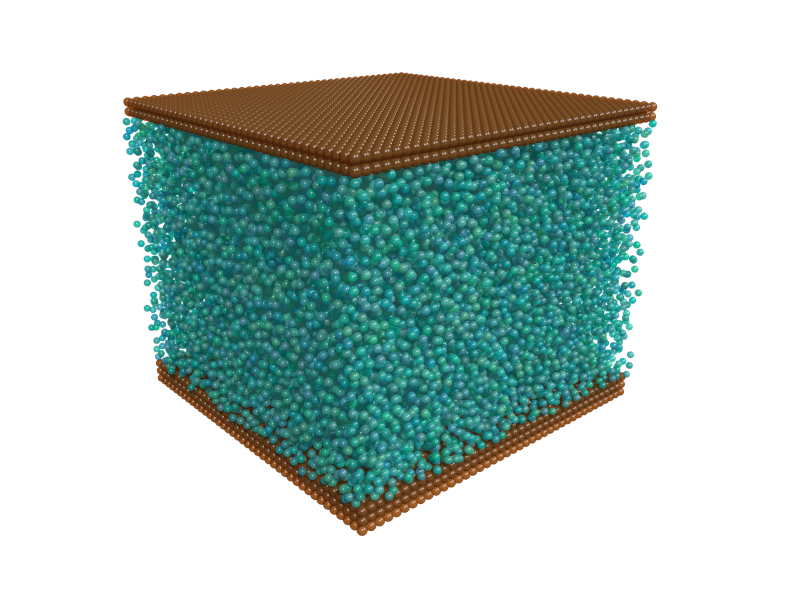
\includegraphics[width=.3\linewidth]{PRL3_gold2_wo_layers_wo_diffuse}
        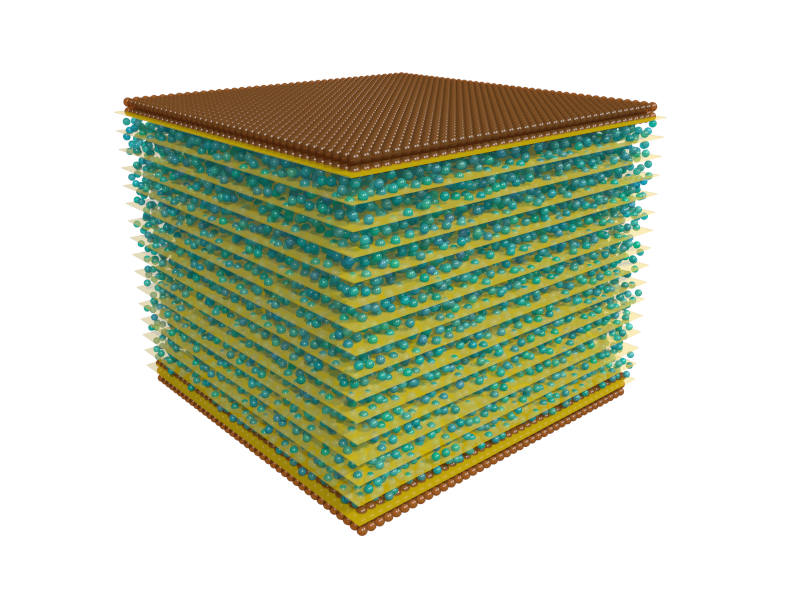
\includegraphics[width=.3\linewidth]{PRL3_gold2_wo_diffuse}
      \end{center}
    \item  Characteristic function $\chi_{\mu}({\bf r})$ and finite element linear basis function $\Phi_{\mu}({\bf r})$
    \begin{align}
    \chi_\mu({\bf r})&=\theta(z_{\mu+ 1}-z)\theta(z-z_\mu)=\chi_\mu(z)
    \nonumber
    \end{align}
    \begin{align}
      \Phi_\mu({\bf r})=\chi_\mu(z)\frac{z_{\mu+1}-z}{\Delta z}+\chi_{\mu-1}(z)\frac{z-z_{\mu-1}}{\Delta z}
      \nonumber
    \end{align}
    \begin{center} 
      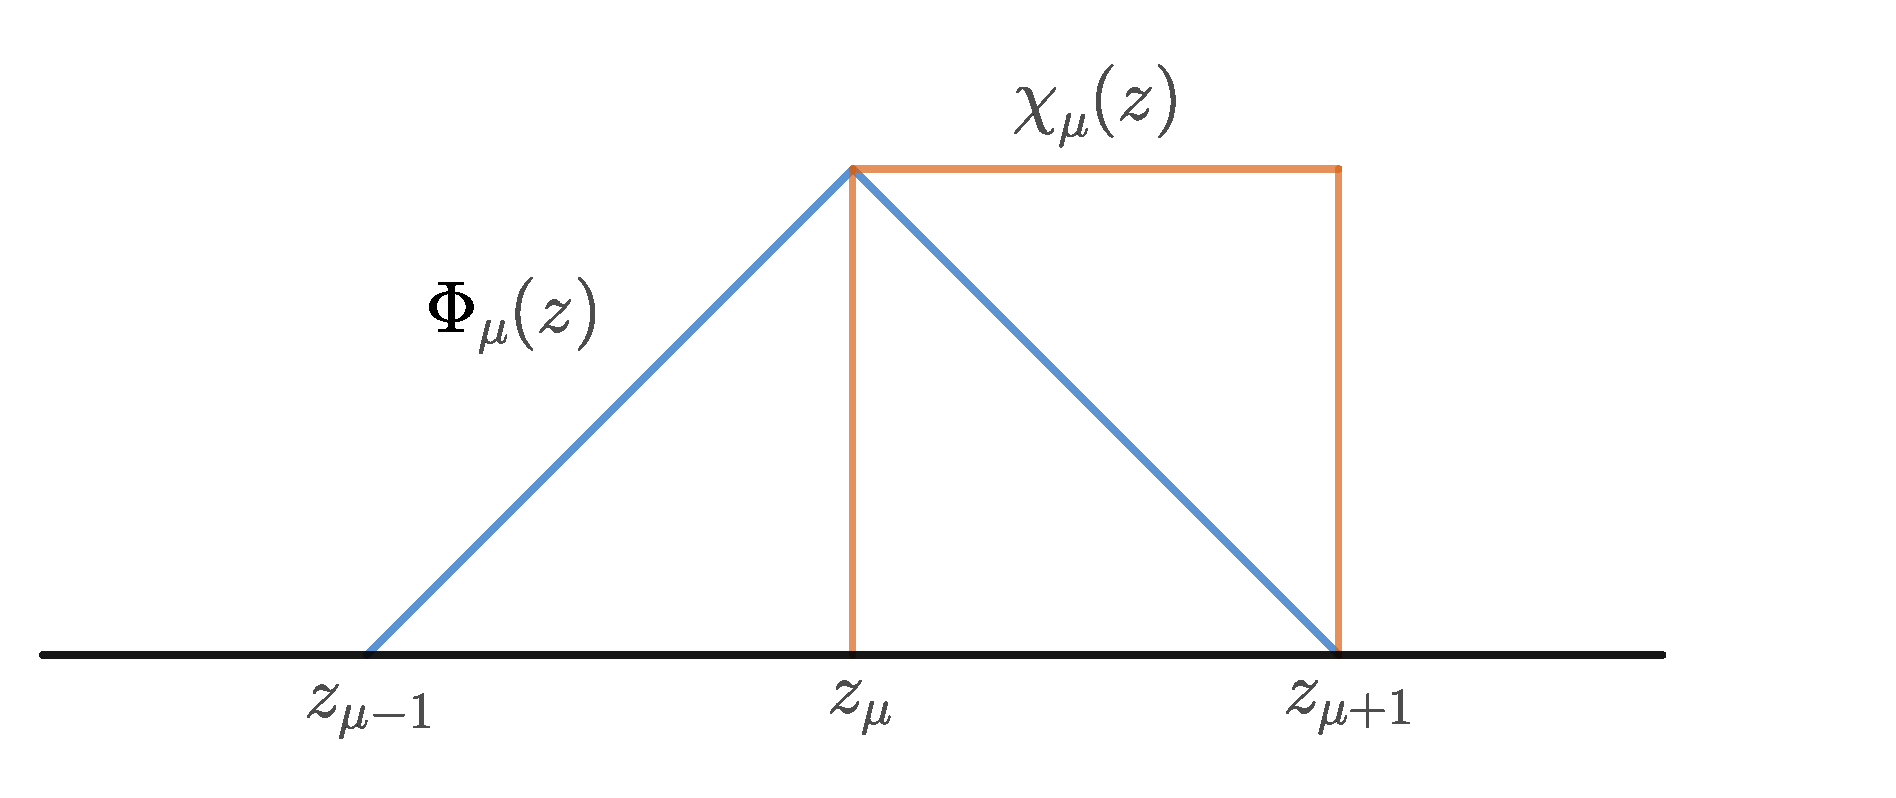
\includegraphics[scale=0.16]{psichi}
    \end{center}
  \end{itemize}
\end{frame}

\begin{frame}{Mass matrix and dual basis functions}
  \begin{itemize}
    \item The usual mass matrix of the finite element method is
      \begin{align}
      M^\Phi_{\mu\nu}&=\llg\Phi_\mu\Phi_\nu\rlg  
      \nonumber
      \end{align}
      where we have introduce the notation $\llg\cdots\rlg=\int d{\bf r}...$
    \item We introduce the discrete velocity field in terms of $M^\Phi_{\mu\nu}$
      \begin{align}
        \tilde{{\bf v}}_{\mu}=\sum_{\nu}{\cal V}_{\mu}[M^{\Phi}]^{-1}_{\mu\nu}{\bf v}_{\nu}
        \nonumber
      \end{align}
  \item We can contruct continuum and discrete fields from dual basis functions $\delta_{\mu}({\bf r})$ and $\psi_\mu({\bf r})$ 
    \begin{align}
      v_\mu=\int d{\bf r}v({\bf r})\delta_\mu({\bf r}),&&
        \overline{v}({\bf r}) =\sum_{\mu}v_\mu\psi_\mu({\bf r})
    \nonumber
    \end{align}
  \end{itemize}
\end{frame}

\begin{frame}{Discrete equations of nanohydrodynamics}
\begin{align}
  \frac{d}{dt}\rho_\mu&=  {\color{blue} \llg\overline{\rho} \; \overline{\bf v}\boldsymbol{\nabla}\delta_\mu \rlg}
\nonumber\\
\frac{d}{dt}{\bf g}_\mu&=
{\color{blue} \llg\overline{\rho} \overline{\bf v}\;\overline{\bf v}\esc\boldsymbol{\nabla}\delta_{\mu}\rlg
-\sum_\nu\llg\overline{\rho}\delta_{\mu}\boldsymbol{\nabla}\delta_{\nu}\rlg
\frac{\partial  F}{\partial \rho_{\nu}}(\rho)}
\nonumber\\
&{\color{red}-\sum_{\nu}{\cal V}_\nu \frac{{\bf n}\esc\left[\boldsymbol{\eta}_{\mu\nu}-\boldsymbol{\eta}_{\mu-1\nu}-\boldsymbol{\eta}_{\mu\nu-1}+\boldsymbol{\eta}_{\mu-1\nu-1}\right]}{\Delta z^2}:{\bf n}\tilde{\bf v}_\nu}
\nonumber\\
&{\color{red}+\sum_{\nu}{\cal V}_\nu\frac{\left[{\bf G}_{\mu\nu}-{\bf G}_{\mu\nu-1}\right]}{\Delta z}\esc{\bf n}\tilde{\bf v}_\nu}
\nonumber\\
&{\color{red}+\sum_{\nu}{\cal V}_\nu\frac{{\bf n}\esc\left[{\bf H}_{\mu\nu}-{\bf H}_{\mu-1\nu}\right]}{\Delta z}\esc\tilde{\bf v}_\nu}
\nonumber\\
&{\color{red}-\sum_{\nu}{\cal V}_\nu\boldsymbol{\gamma}_{\mu\nu}\esc\tilde{\bf v}_\nu}
\nonumber
\end{align}
\end{frame}

\begin{frame}{Symmetry assumptions}
  \begin{itemize}
    \item The system is isotropic when we rotate it with respect to an axis perpendicular to the walls...
    \item ... and reflect it with respect to a plane containing the axis. 
    \item Large simplification of the structure of the tensors $\boldsymbol{\eta}_{\mu\nu}$, ${\bf G}_{\mu\nu}$, ${\bf H}_{\mu\nu}$ and $\boldsymbol{\gamma}_{\mu\nu}$.
    \item Under the simplification we may separate the evolution of the selected variables in two contribution: normal and tangent.
    \end{itemize}
\end{frame}

\begin{frame}{Normal and tangent evolution}
\begin{itemize}
  \item The normal evolution 
\begin{align}
  \frac{d}{dt}\rho_\mu=&  {\color{blue} \llg\overline{\rho} \; \overline{v}^{z}{\nabla}^{z}\delta_\mu \rlg}
\nonumber\\
    \frac{d}{dt}{{\bf g}}^{z}_\mu=&
{\color{blue} \llg\overline{\rho}\; \overline{v}^{z}\;\overline{v}^{z}{\nabla}^{z}\delta_{\mu}\rlg
-\llg\overline{\rho}\delta_{\mu}{\nabla}^{z}\delta_{\nu}\rlg
\frac{\partial  F}{\partial \rho_{\nu}}(\rho)}
{\color{red} +M_{\mu\nu}^{\bot}{\cal V}_\nu\tilde{v}^{z}_\nu}
\nonumber
\end{align}
  \item The parallel evolution for $\alpha=x,y$  
\begin{align}
  \frac{d}{dt}{{\bf g}}^\alpha_\mu=&{\color{red}-M_{\mu\nu}^{||}{\cal V}_\nu\tilde{v}^\alpha_\nu}
\nonumber
\end{align}
\item The dissipative matrix for $\odot=||,\bot$
\begin{align}
M^{\odot}_{\mu\nu} 
=&-\frac{\eta^{\odot}_{\mu\nu}-\eta^{\odot}_{\mu-1\nu}-\eta^{\odot}_{\mu\nu-1}+\eta^{\odot}_{\mu-1\nu-1}}{\Delta z^2}
+\frac{{G}^{\odot}_{\mu\nu}-{G}^{\odot}_{\mu\nu-1}}{\Delta z} \nonumber \\
&+\frac{{H}^{\odot}_{\mu\nu}-{H}^{\odot}_{\mu-1\nu}}{\Delta z}
-{\gamma}^{\odot}_{\mu\nu}
\nonumber
\end{align}
\end{itemize}
\end{frame}

\begin{frame}{The discrete transport kernels}
\begin{align}
\eta^{||}_{\mu\nu}&
=\frac{1}{k_BT}\int_0^\tau  dt\left\langle 
{\cal Q}\hat{\boldsymbol{\sigma}}^{xz}_\mu(t){\cal Q}\hat{\boldsymbol{\sigma}}^{xz}_\nu
\right\rangle&&
%\nonumber\\
\eta^{\bot}_{\mu\nu}
= \frac{1}{k_BT}\int_0^\tau  dt\langle 
{\cal Q}\hat{\boldsymbol{\sigma}}^{zz}_\mu(t)
{\cal Q}\hat{\boldsymbol{\sigma}}^{zz}_\nu\rangle
\nonumber\\
G^{||}_{\mu\nu}&
=\frac{1}{k_BT} \int_0^\tau  dt
\left\langle{\cal Q}\hat{\bf F}^{x}_\mu(t)
{\cal Q}\hat{\boldsymbol{\sigma}}^{xz}_\nu
\right\rangle&&
%\nonumber\\
G^{\bot}_{\mu\nu}=\frac{1}{k_BT} \int_0^\tau  dt
\left\langle {\cal Q}\hat{\bf F}^{z}_\mu(t)
{\cal Q}\hat{\boldsymbol{\sigma}}^{zz}_\nu
\right\rangle
\nonumber\\
H^{||}_{\mu\nu}&
=\frac{1}{k_BT} 
\int_0^\tau  dt
\left\langle{\cal Q}\hat{\boldsymbol{\sigma}}^{xz}_\mu(t){\cal Q}\hat{\bf F}^{x}_\nu\right\rangle&&
%\nonumber\\
H^\bot_{\mu\nu}=\frac{1}{k_BT} 
\int_0^\tau  dt\left\langle {\cal Q}\hat{\boldsymbol{\sigma}}^{zz}_\mu(t){\cal Q}\hat{\bf F}^{z}_\nu\right\rangle
\nonumber\\
\gamma^{||}_{\mu\nu}&=
\frac{1}{k_BT} \int_0^\tau  dt
\left\langle 
{\cal Q}\hat{\bf F}^{x}_\mu(t)
{\cal Q}\hat{\bf F}^{x}_\nu\right\rangle&&
%\nonumber\\
\gamma^{\bot}_{\mu\nu}=
\frac{1}{k_BT} \int_0^\tau  dt\left\langle 
{\cal Q}\hat{\bf F}^{z}_\mu(t){\cal Q}\hat{\bf F}^{z}_\nu
\right\rangle
\nonumber
\end{align}
\end{frame}

\begin{frame}{Summary}
  \begin{itemize}
    \item 
    \item We have obtained a set of nonlocal transport coefficients that are include in the nanohydrodynamic equations.
    \end{itemize}
\end{frame}

\section{Space and time locality for unconfined fluids}
\begin{frame}{Mori's theory}
  \begin{itemize}
    \item Linear dynamic equations not only for the averages of the relevant variables but also for their correlations
\begin{align}
  \frac{d}{dt}C(t)&=-L\esc C^{-1}(0)\esc C(t)
  -{\color{red}\int_0^tdt' \Gamma(t-t')\esc C^{-1}(0)\esc  C(t')}
\nonumber
\end{align}
where the following matrices have been introduced
\begin{align}
  L&=\langle \hat{A}i{\cal L}\hat{A}^T\rangle \nonumber \\
  C(0)&=\langle \hat{A}\hat{A}^T\rangle \nonumber \\
\Gamma(t)&=\langle F^+(t)F^{+T}(0)\rangle
\nonumber
\end{align}
\item The projected forces are given by
\begin{align}
F^+(t)&= \exp\{{\cal Q}i{\cal L}t\} {\cal Q}i{\cal L}\hat{A}  
\nonumber
\end{align}
\item ${\cal Q}=1-{\cal P}$ where  ${\cal P}$  is Mori's  projector 
\begin{align}
  {\cal P}\hat{F}(z) = \langle \hat{F}\rangle+ \langle \hat{F}\hat{A}^T \rangle\esc  C^{-1}(0)\esc  \hat{A}(z)
\nonumber
\end{align}
\end{itemize}
\end{frame}

\begin{frame}{Markovian approximation}
  \begin{itemize}
    \item Memory-less term 
  \begin{align}
{\color{red}\int_0^tdt' \Gamma(t-t')\esc C^{-1}(0)\esc  C(t')} \simeq M^* C^{-1}(0)C(t)
\nonumber
\end{align}
\item Expression for the correlations
\begin{align}
  \frac{d}{dt}C(t) &= - (L+M^*)\esc C^{-1}(0)\esc C(t) \nonumber \\
                     &\equiv \Lambda^*\esc C(t)
  \nonumber
\end{align}
\item For a linear Markovian theory the only possibility for a correlation is to decay in an exponential matrix way
\begin{align}
  C(t)=\exp\{-\Lambda^* (t-\tau)\}\esc C(\tau)
\nonumber
\end{align}
\item {\bf We need to find a constant matrix $\boldsymbol{\Lambda^*}$}.
\end{itemize}
\end{frame}

\begin{frame}{Simpler case: unconfined fluid}
  \begin{center}
  \begin{itemize}
  \item The system
  \begin{figure}
    \includegraphics[width=0.5\linewidth]{temp_wo_walls}
    \includegraphics[width=0.5\linewidth]{temp_wo_walls_w_layers2}
\end{figure}
\item The relevant variable
\begin{align}
  \hat{\bf g}_\mu(z)= \sum_i^N{\bf p}_i\delta_\mu({\bf r}_i)
%  i{\cal L}  \hat{g}_{\mu}(z)=-\frac{\hat{\sigma}^{xz}_{\mu}-\hat{\sigma}^{xz}_{\mu-1}}{\Delta z}
\nonumber
\end{align}
\end{itemize}
  \end{center}
\end{frame}

 \begin{frame}{Simulation set up}
   \begin{itemize}
     \item Simulation of $28749$ particles interacting with a LJ potential truncated at $\sigma=2.5$.
     \item Box size $40x40x30$.
     \item $dt=0.002$ in reduced units.
     \item Equilibration stage
       \begin{itemize}
         \item Langevin thermostat for $10^5$ timesteps: $T=2.0$, $\rho=0.6$.
         \item NVE microcanonical conditions for a further $10^5$ timesteps.
          \end{itemize}
        \item Production stage
       \begin{itemize}
         \item $1.5\times10^6$ timesteps.
         \item $z$ axis binned in $60$ bins $\mu$. {$\boldsymbol{\Delta} {\bf z=0.5}\boldsymbol{\sigma}$}.
         \item $g_{\mu}^x(t)$ recorded every $10$ timesteps.
         \end{itemize}
     \end{itemize}
 \end{frame}

 \begin{frame}{Building the correlation matrix $C(t)$}
\begin{figure}[h!]
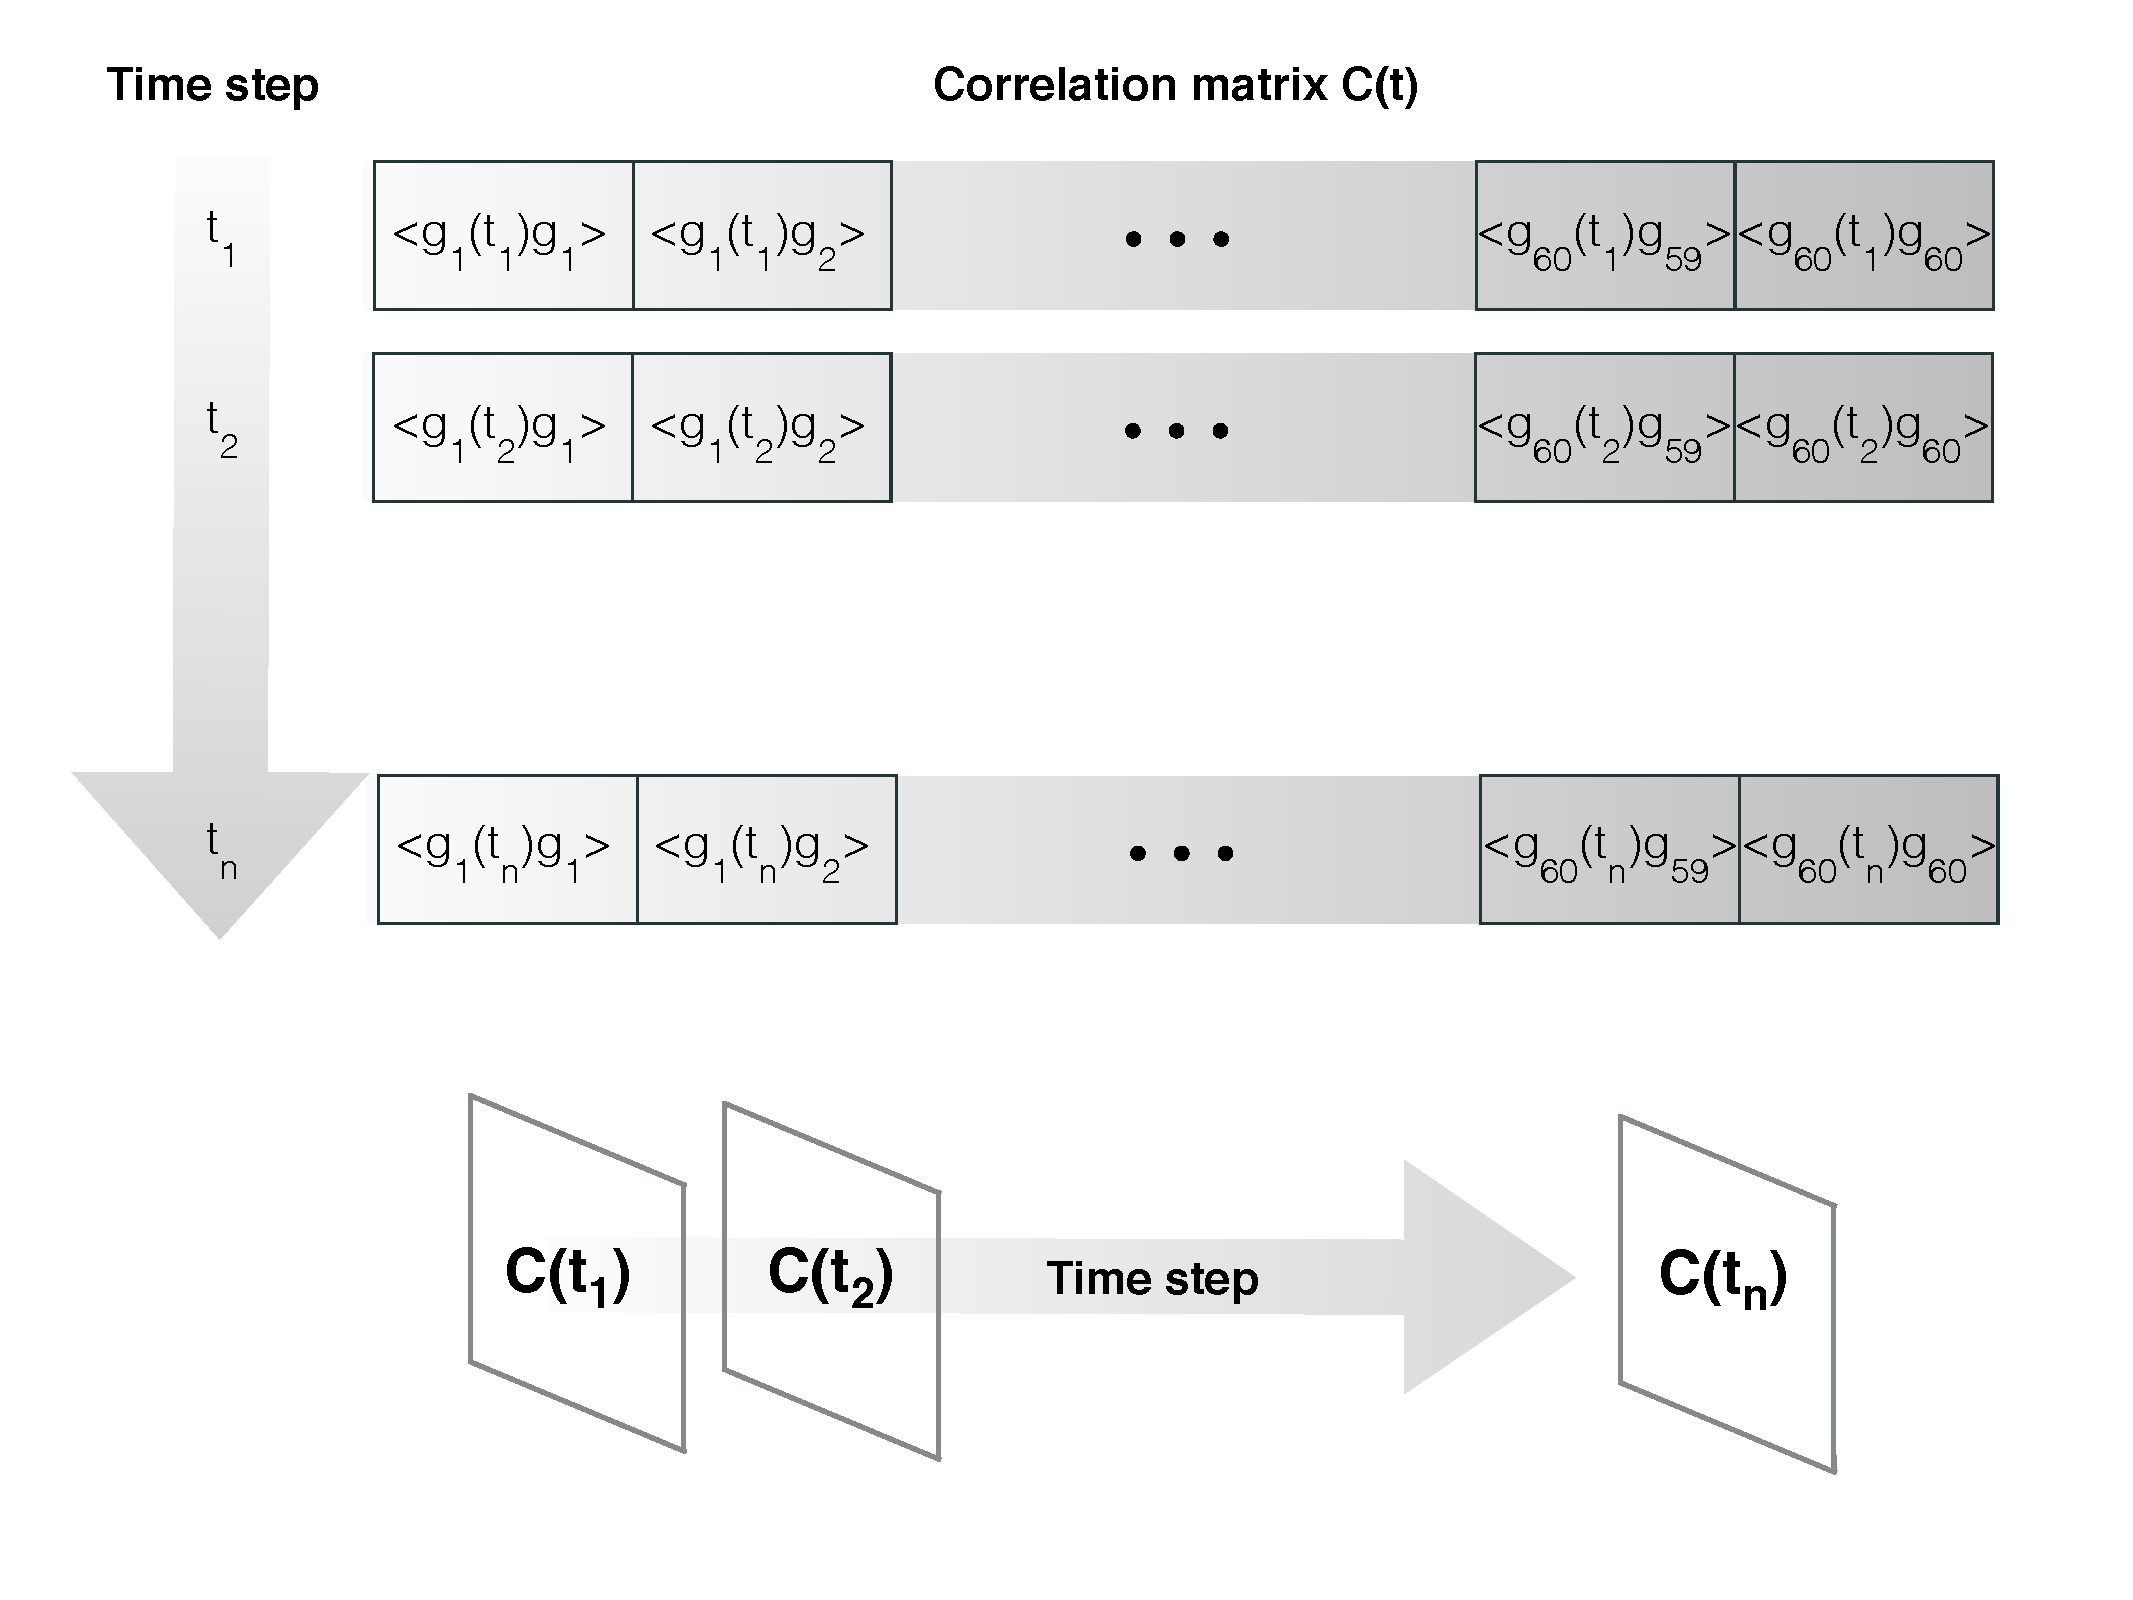
\includegraphics[width=\linewidth]{lammps-python}
\end{figure}
 \end{frame}
 
 \begin{frame}{The correlation matrix $C(t)$ and its eigenvalues $\tilde{C}_{\mu\mu}$}
   \begin{itemize}
 \item
   The correlation matrix $C(t)$ at $t=0$ (left) and $t=0.6$ (right)
\begin{figure}[h!]
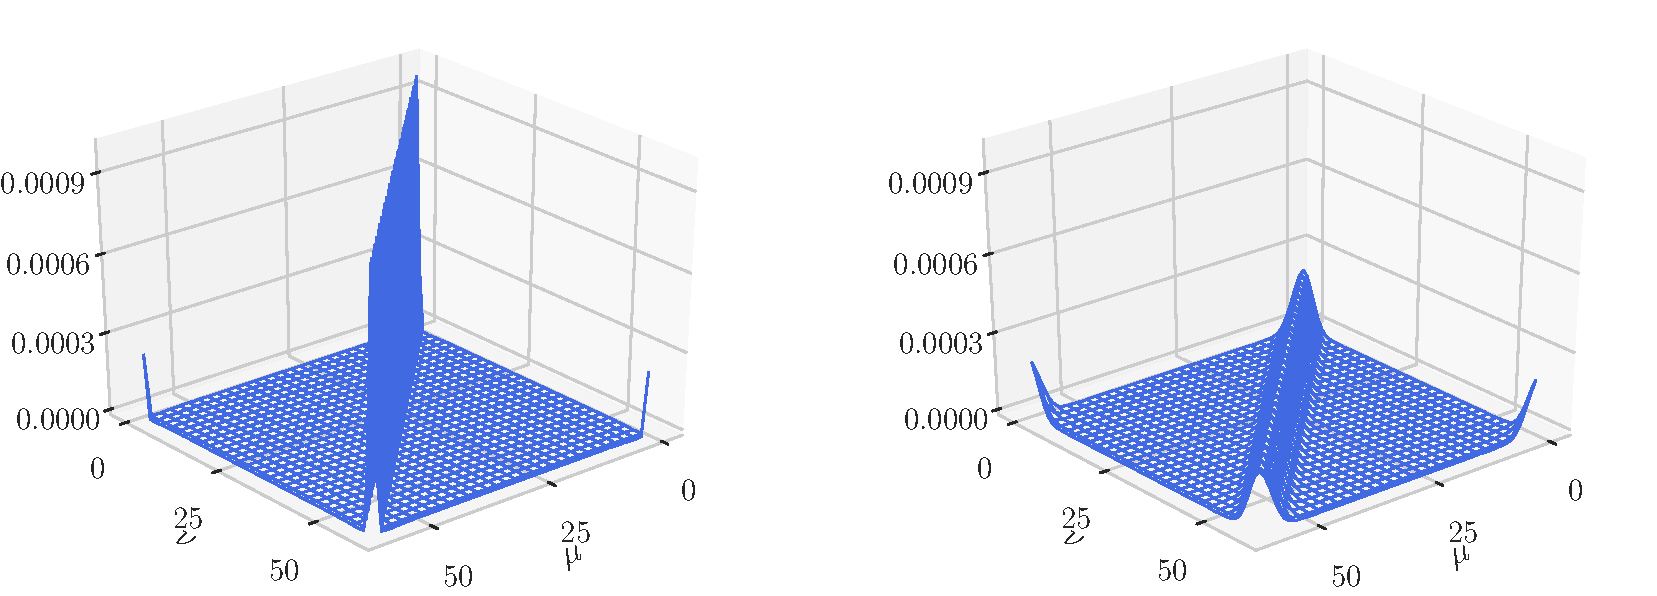
\includegraphics[width=\linewidth]{Ct-matrix-PBC}
\end{figure}
\item  The evolution of the different eigenvalues $\tilde{C}_{\mu\mu}(t)$. %The horizontal  line  at  the   value  $2\times10^{-5}$,  signaling  the
  %threshold below which statistical errors give spurious results.
\begin{figure}[h!]
  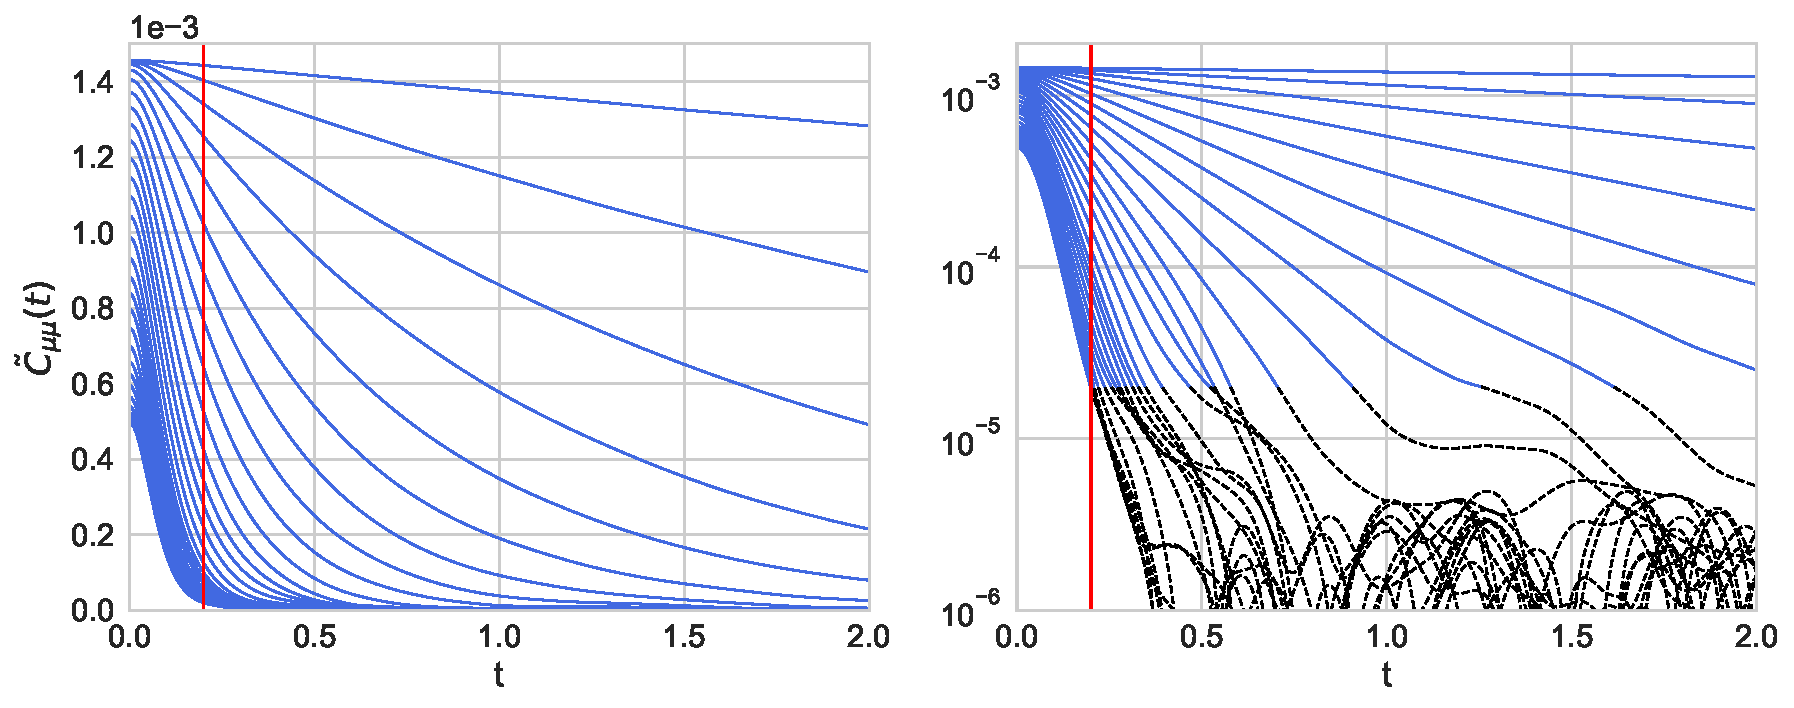
\includegraphics[width=\linewidth]{CtFourier-PBC-exp}
\end{figure}
\end{itemize}
\end{frame}

\begin{frame}{Validation of the Markovian approximation}
\begin{figure}[h!]
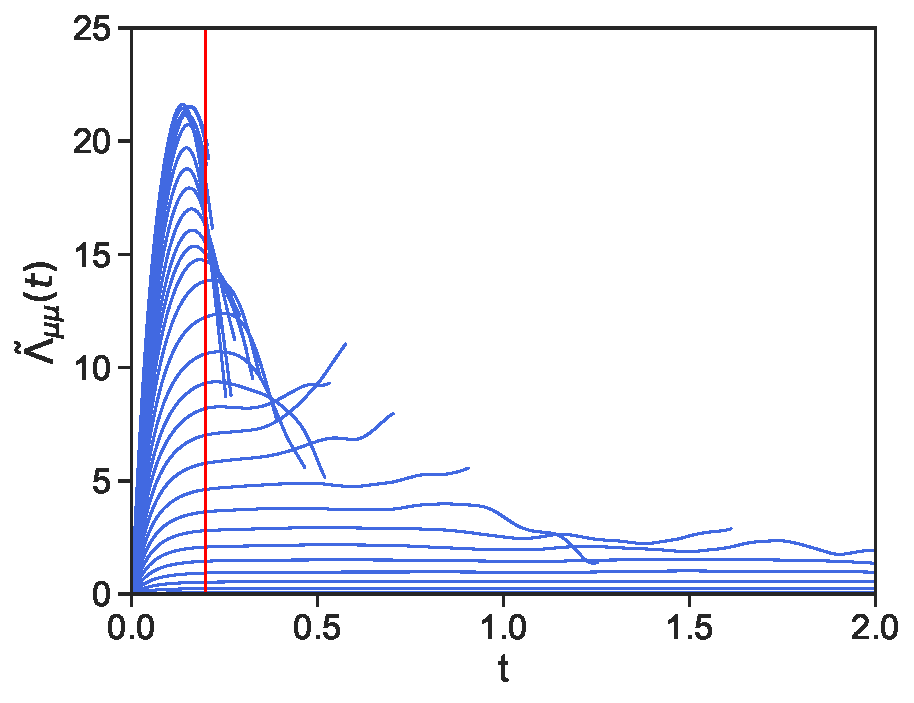
\includegraphics[width=\linewidth]{LambdatFourier-PBC-defense}
\end{figure}
In  the left  panel, in
  ascending  order the  plotted times  go  from $t=0$  to $t=0.20$  in
  intervals of $0.02$.  In the right pannel the time evolution of $\tilde{\Lambda}_{\mu\mu}(t)$.
\end{frame}

\section{Markovian behaviour near solids}
\begin{frame}
\begin{itemize}
  \item The system
\begin{figure}
    \centering
    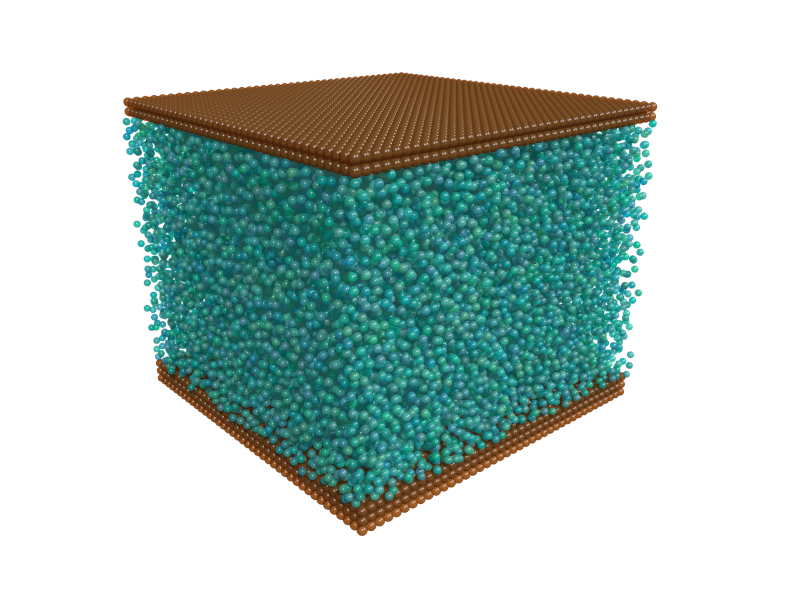
\includegraphics[width=0.45\linewidth]{PRL3_gold2_wo_layers_wo_diffuse}
    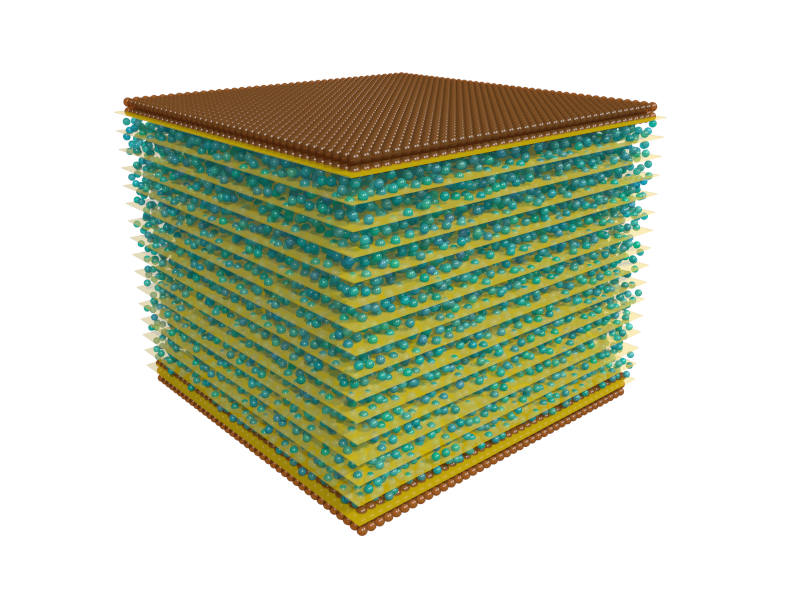
\includegraphics[width=0.45\linewidth]{PRL3_gold2_wo_diffuse}
\end{figure}
\item The CG variable and its correlation
\begin{align}
  \hat{\bf g}^x_\mu= \sum_i^N{\bf p}_i\delta_\mu({\bf q}_i), && 
  \hat{g}^T=(\hat{\bf   g}^x_1,\cdots,\hat{\bf  g}^x_{N_{\rm   bin}}), &&
  C(t)=\llangle \hat{g}(t) \hat{g}^T\rrangle 
\nonumber
\end{align}
\end{itemize}
\end{frame}

\begin{frame}{Simulation set up}
   \begin{itemize}
     \item Simulation of $28175$ fluid particles interacting with a LJ potential truncated at $\sigma=2.5$.
     \item Two solid walls in the $xy$ plane confine the fluid.  
     \item Box size $40x40x33$. 
     \item $dt=0.002$ in reduced units.
     \item Equilibration stage
       \begin{itemize}
         \item Langevin thermostat for $10^5$ timesteps: $T=2.0$, $\rho=0.6$.
         \item NVE microcanonical conditions for a further $10^5$ timesteps.
          \end{itemize}
        \item Production stage
       \begin{itemize}
         \item $12\times10^6$ timesteps.
         \item $z$ axis binned in $66$ bins $\mu$ $\boldsymbol{\Delta} {\bf z=0.5}\boldsymbol{\sigma}$ or $33$ bins $\mu$ $\boldsymbol{\Delta} {\bf z=2} \boldsymbol{\sigma}$.
         \item $g_{\mu}^x(t)$ recorded every $2$ timesteps. 
         \end{itemize}
     \end{itemize}
\end{frame}

\begin{frame}{Reciprocal space}
  \begin{itemize}
    \item Eigenvalues $\tilde{C}_{\mu}$ and eigenvectors $u_{\mu}$
\begin{align}
  C(t)&=\sum_\mu^{N_{\rm bin}}\tilde{C}_\mu(t) u_\mu(t) \otimes u_\mu^T(t)
\nonumber
\end{align}
    \item Unitary matrix $E(t)$
\begin{align}
  E^{-1}(t)\esc C(t)\esc E(t)=\tilde{C}(t)
\nonumber
\end{align}
\item We observed that $\dot{E}\simeq 0$.
\item The predictions of $C(t)$ in the reciprocal space
\begin{align}
  \tilde{C}_\mu(t)&=\exp\{-\tilde{\Lambda}_{\mu\mu} (t-\tau)\}  \tilde{C}_\mu(\tau)
  \nonumber
\end{align}
    \end{itemize}
\end{frame}

\begin{frame}{Thin bins ($\Delta z=0.5\sigma$)}
  \begin{itemize}
    \item $C_{\mu\nu}(t)$ for  $t=0$ (left) and $t=0.6$ (right).
\begin{figure}[h!]
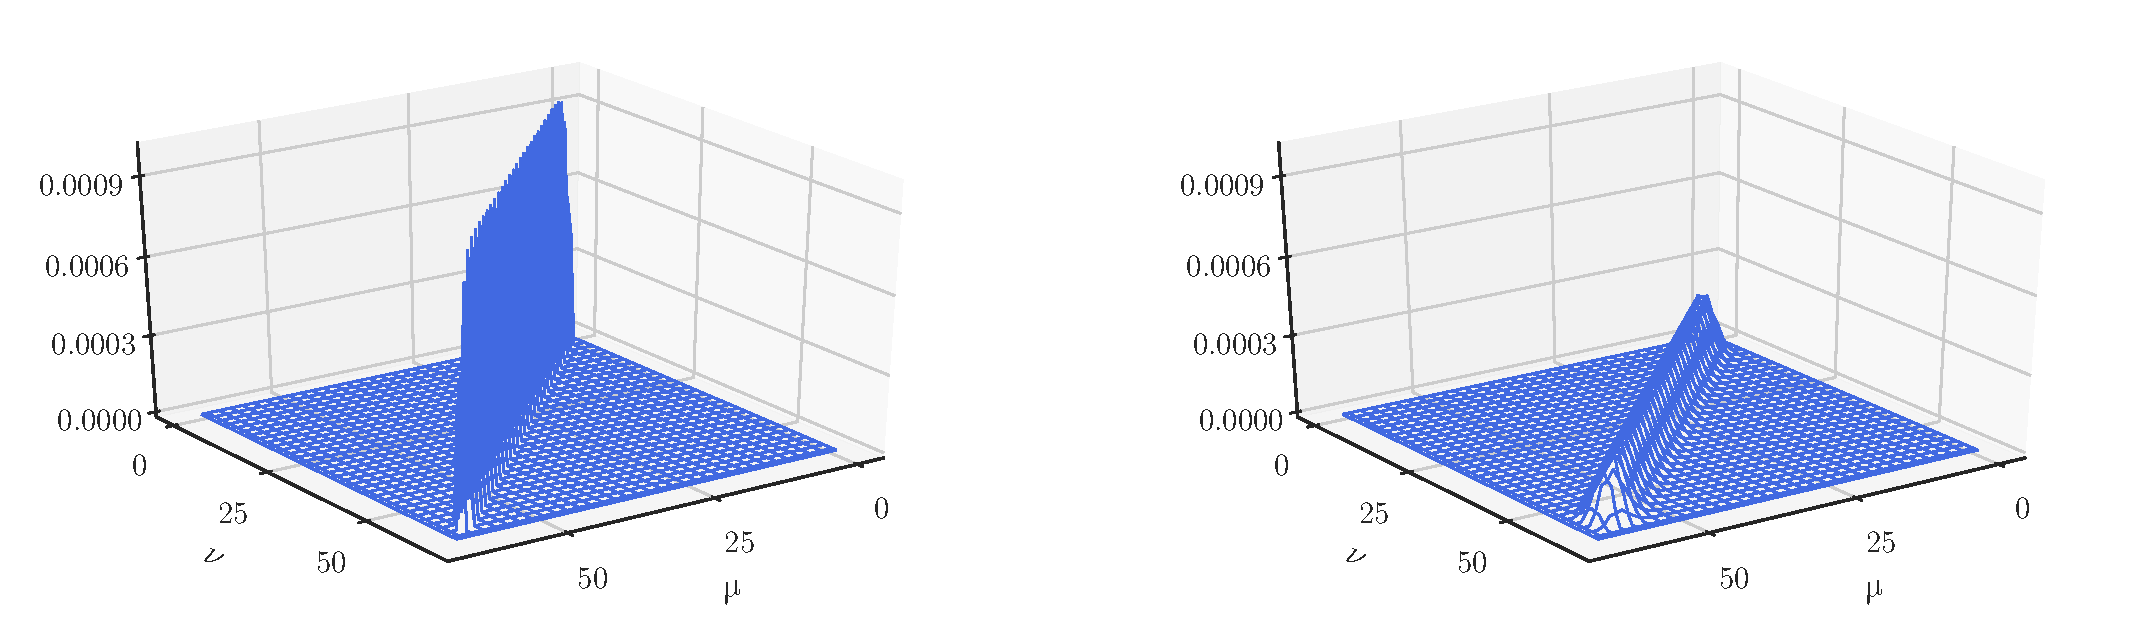
\includegraphics[width=\linewidth]{Ct-matrix-WALLS-66nodes}
\end{figure}
\item Evolution of different eigenvalues $\tilde{C}_{\mu\nu}(t)$
\begin{figure}[h!]
  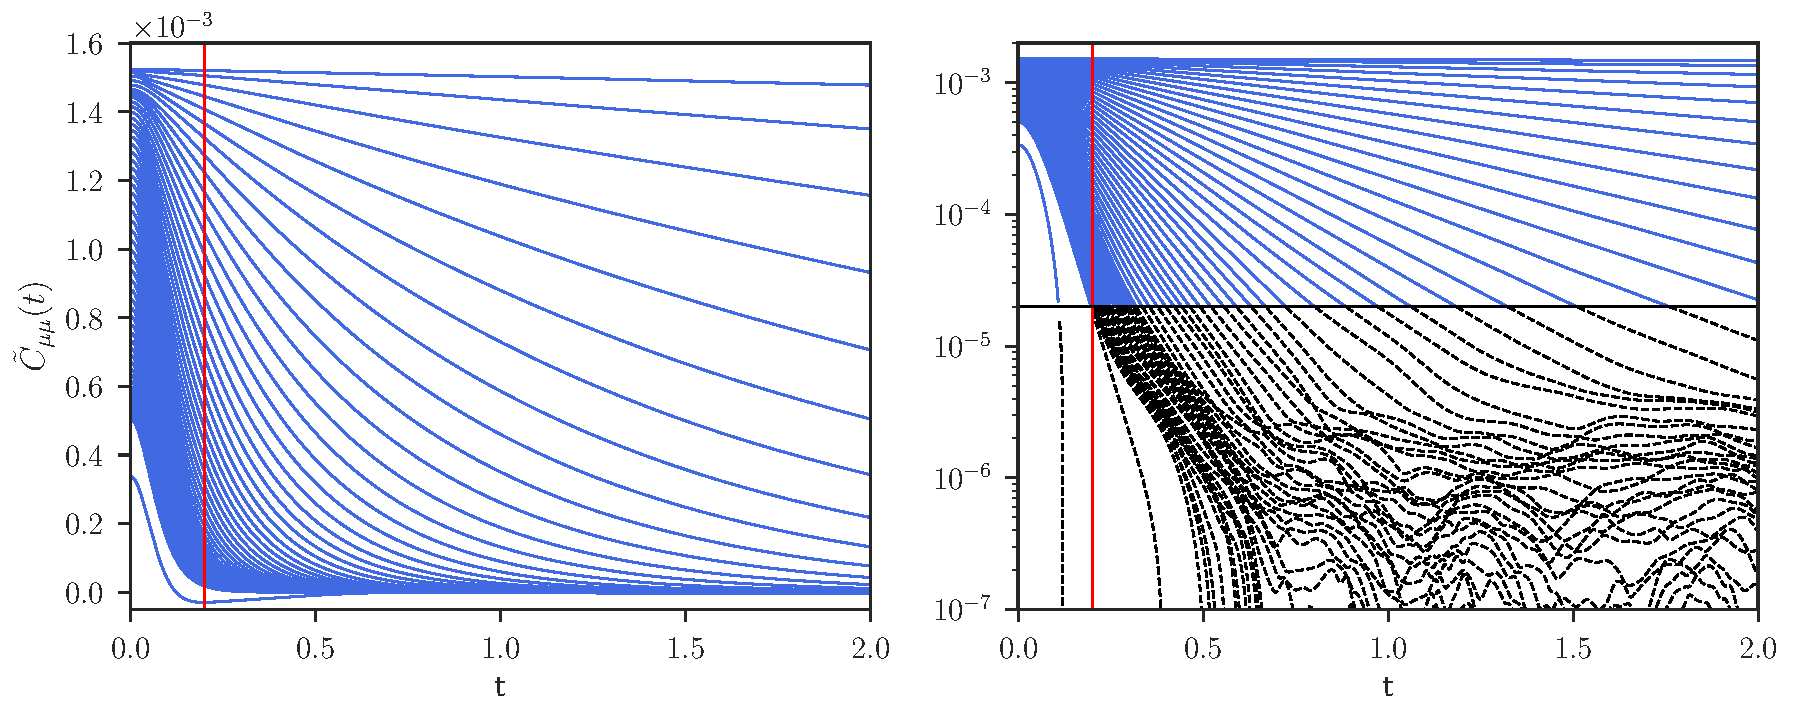
\includegraphics[width=\linewidth]{CtRec-WALLS-66nodes-exp}
\end{figure}
\end{itemize}
\end{frame}

\begin{frame}{$\tilde{\Lambda}(t)$ ($\Delta z=0.5\sigma$)}
Diagonal elements  $\tilde{\Lambda}_{\mu\mu}(t)$ of $\Lambda(t)$ in the reciprocal space. After a time $\tau=0.2$ we observe a nice plateau for the lower modes. 
\begin{figure}[h!]
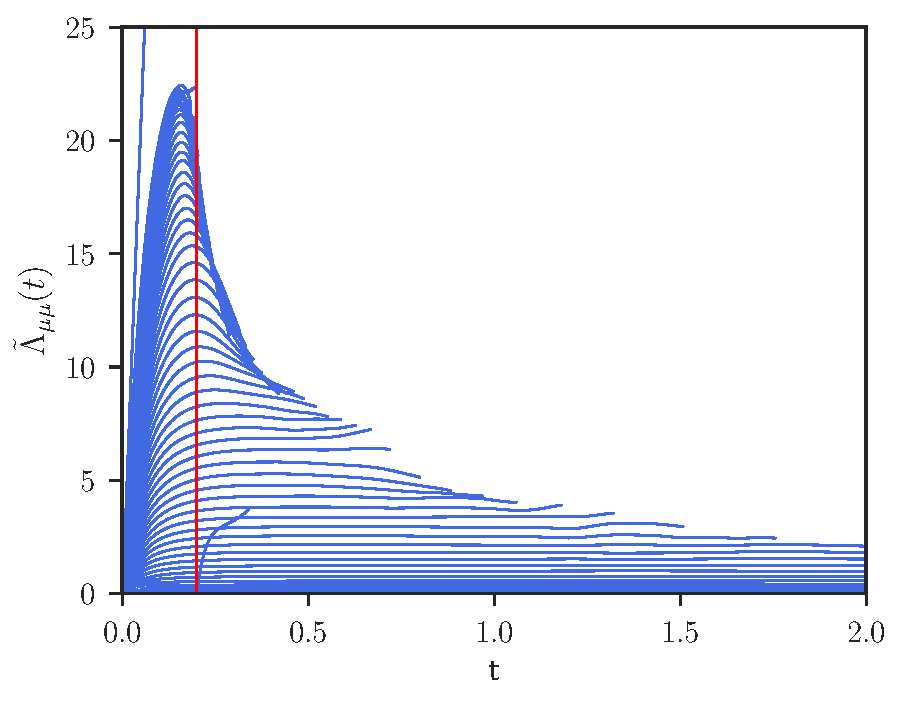
\includegraphics[width=0.5\linewidth]{LambdatRec-WALLS-66nodes}
\end{figure}
\end{frame}

\begin{frame}{Eigenvalues and eigenvectors near the walls ($\Delta z=0.5\sigma$)}
    The eigenvalues $\tilde{C}_{\mu}(t)$ of the correlation matrix $C(t)$ for $\mu=59,60$ which are identical and superimpose (left) and the corresponding eigenvectors $u_{\mu}$ in blue and orange, respectively (right).
  \begin{figure}[h!]
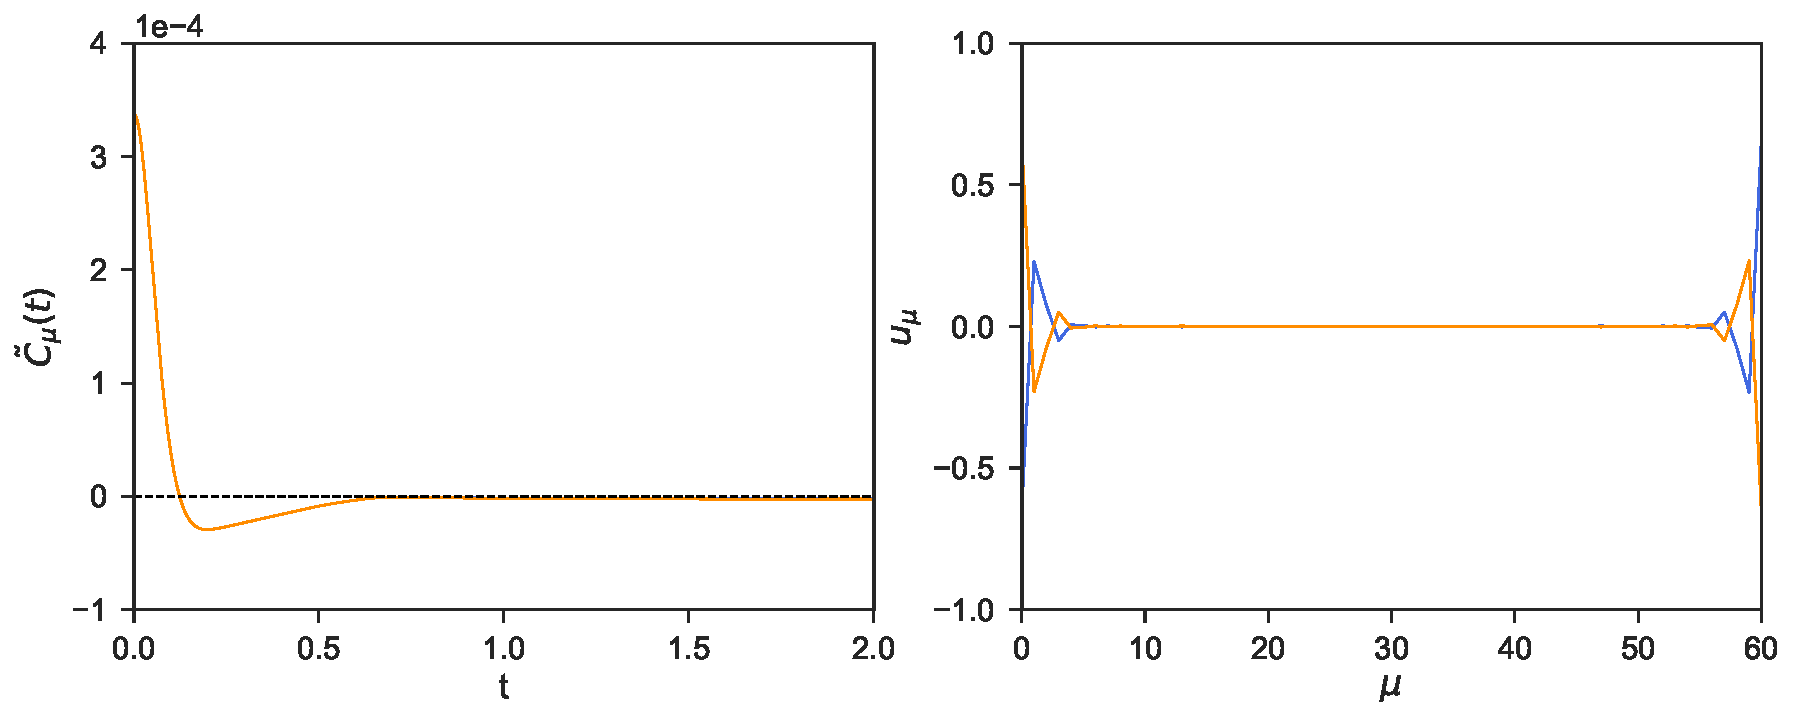
\includegraphics[width=0.5\linewidth]{EigenvaluesVectors-WALLS-66nodes}
\end{figure}
\end{frame}

\end{document}
